\chapter{Bankruptcy, Solvency and Hindsight}
\label{ch:bankruptcy}

\section{The question bankruptcy courts ask}

When a firm fails, its creditors look backwards. A leveraged buyout two years earlier paid hundreds of millions of dollars to the old shareholders and loaded the company with debt. A dividend was paid shortly before the collapse. A parent company sold a subsidiary to the debtor at a high price, or took its assets for a low one. Bankruptcy law lets a trustee or creditors' committee claw back such transfers if they were fraudulent, either because they were made with actual intent to hinder, delay or defraud creditors, or because they were constructively fraudulent: made for less than reasonably equivalent value at a time when the debtor was insolvent, was left with unreasonably small capital, or intended or believed it would incur debts beyond its ability to pay. Section 548 of the United States Bankruptcy Code states these tests, and state law versions under the Uniform Fraudulent Transfer Act and its successor, the Uniform Voidable Transactions Act, are available to the trustee through section 544(b). English law has analogous provisions on transactions at an undervalue and preferences in the Insolvency Act 1986.\index{fraudulent transfer}\index{solvency tests}

Each of the financial tests is a statement about the future made at a moment in the past. Was the debtor insolvent on the date of the transfer, meaning that the fair value of its assets was less than its debts? Was its capital unreasonably small for the business it was about to conduct? Would it be able to pay its debts as they matured? None of these can be answered by looking at what later happened, since the firm's failure is the reason the question is being asked, and a court that reasons from the failure to the earlier insolvency commits the error of hindsight. Each must be answered with the information available at the time. That makes solvency a probability judgment conditioned on a past information set, and it makes bankruptcy litigation a natural home for Bayesian reasoning.

J. B. Heaton, a Chicago lawyer and financial economist with whom one of us has also written on deep learning in finance \citep{heaton2017}, has argued that legal solvency tests should be understood through financial economics, and that the right test depends on the context in which it is applied \citep{heaton2002,heaton2007}. This chapter develops his argument in Bayesian terms and works through the principal cases.

\section{Three tests as three posteriors}

\subsection{The balance sheet test}

The balance sheet test asks whether the fair value of the debtor's assets exceeded its liabilities. Fair value is not book value: it is what the assets would fetch in an orderly sale, or the value of the business as a going concern. For a firm whose assets are its future cash flows, fair value is the present value of those cash flows, which depends on forecasts. In financial economics the natural measure is the market value of the firm's enterprise, the sum of the market values of its debt and equity.\index{balance sheet test}

Heaton's first point is that the balance sheet test, read literally, asks the wrong question for a going concern. A firm whose enterprise value is slightly below the face value of its debt is not necessarily doomed. Its equity still has value as an option on the upside, and creditors may be paid in full if things go well. Conversely, a firm whose enterprise value exceeds its debt may face a high probability of default if its assets are volatile. What matters to creditors is the probability and severity of default, not a point comparison of two numbers.

\subsection{The Merton model}

Merton's structural model of credit risk makes this explicit \citep{merton1974}. Let $V_t$ be the value of the firm's assets at time $t$. Treat the firm's assets as following a geometric Brownian motion with volatility $\sigma$, and its debt as a single zero coupon bond with face value $D$ maturing at $T$. Equity is a call option on the assets with strike $D$. The probability, under the real world measure with drift $\mu$, that the firm defaults at $T$ is
\begin{equation}
\Prob(V_T < D) = \Phi\left(-\frac{\log(V_0/D) + (\mu - \sigma^2/2)T}{\sigma\sqrt{T}}\right).
\label{eq:merton}
\end{equation}
Here $\Phi$ is the standard normal cumulative distribution function, the probability that a standard normal variable falls below its argument. Figure~\ref{fig:merton} plots \eqref{eq:merton} as a function of leverage. In the parameterisation of the figure, with an asset drift of three per cent, a firm with debt equal to ninety per cent of asset value has a one year default probability of about one in five if its asset volatility is fifteen per cent, and of nearly one half if it is fifty per cent. The balance sheet test treats both as solvent.\index{Merton model}

\begin{figure}[t]
\centering
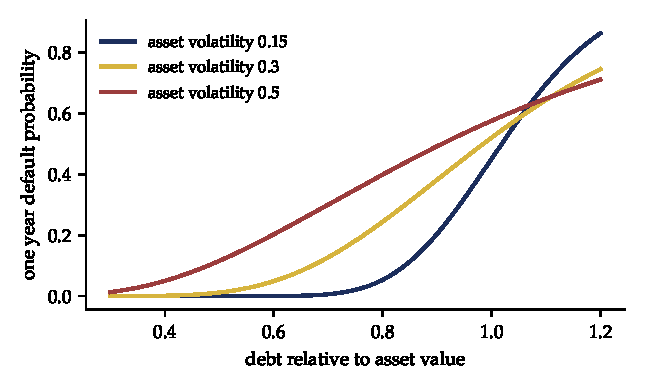
\includegraphics[width=\linewidth]{fig_merton}
\caption{One year default probability in the Merton model as a function of leverage, for three asset volatilities. The balance sheet test draws a line at leverage of one; the probability of default changes smoothly and depends heavily on volatility.}
\label{fig:merton}
\end{figure}

\subsection{Unreasonably small capital and ability to pay}

The unreasonably small capital test and the ability to pay test are forward looking by design. Courts have described the first as asking whether the debtor had sufficient capital to withstand reasonably foreseeable difficulties, and have said that it requires an assessment of the reasonableness of the debtor's projections at the time. In \emph{Moody v Security Pacific Business Credit}, the Third Circuit held that the test looks to the ability to generate sufficient profits to sustain operations, and that projections must be reasonable and prudent when made \citep{moody1992}. In Bayesian terms, both tests ask whether the posterior probability of failing to meet obligations over a relevant horizon, given information at the transfer date, was unacceptably high.

What is unacceptably high? The statute does not say. Heaton argues that this is the right place to recognise that the tests serve different purposes in different contexts. Fraudulent transfer law protects creditors against transfers that shift risk to them without their consent. A transfer that raises the probability of default from one per cent to two per cent harms creditors less than one that raises it from ten to forty. A Bayesian formulation would make the test a threshold on the probability of default, or better, on the expected loss to creditors caused by the transfer, with the threshold set by the purpose of the rule.

\section{Hindsight}

\subsection{The psychology}

Kamin and Rachlinski showed in a well known experiment that people asked to judge whether a precaution should have been taken assess the probability of the harm much higher, and are more ready to find that the precaution was required, when they know the harm occurred \citep{kamin1995}. Subjects who were told only the facts before a flood judged the risk low; subjects told that a flood occurred judged the same risk, on the same prior information, much higher, even when instructed to ignore the outcome. Hindsight bias is robust, and judges are not immune to it \citep{guthrie2001}.\index{hindsight bias}

In fraudulent transfer litigation hindsight pushes every assessor, including the court, towards insolvency. The case exists only because the debtor failed. The trustee's expert, retained after the failure, builds a valuation as of the transfer date, choosing among many reasonable assumptions about growth, margins and discount rates. It is easy, and not necessarily dishonest, to choose assumptions that look reasonable in light of what is now known. The defendant's expert leans the other way, for partisan reasons rather than hindsight. The court must choose between two valuations, each a sample from a distribution of possible expert opinions, both shaped by their authors' knowledge of the outcome.

\subsection{A model of hindsight}

Let $\pi$ be the true ex ante probability of default given the information at the transfer date, and $F$ the event that the firm later failed. An expert who forms an estimate after observing $F$ and who cannot fully disregard it reports
\begin{equation}
\hat\pi = \pi + \beta\,\mathbb{1}_F + \epsilon,
\end{equation}
where $\mathbb{1}_F$ is one if the firm failed and zero otherwise, with $\beta > 0$ measuring hindsight bias and $\epsilon$ noise. Because the cases that reach court are exactly those with $F = 1$, the court sees $\hat\pi = \pi + \beta + \epsilon$. There are two distortions. The estimate is biased upwards by $\beta$. And the distribution of $\pi$ among litigated cases is itself shifted upwards relative to all transactions, because failure is more likely when $\pi$ is high, which is a selection effect, not a bias: firms that failed did on average have higher ex ante risk. Figure~\ref{fig:hindsight} illustrates the first. A court needs to correct for the first without overcorrecting for the second.

\begin{figure}[t]
\centering
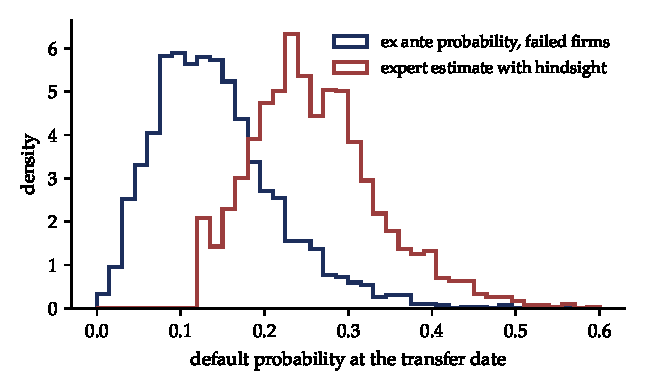
\includegraphics[width=\linewidth]{fig_hindsight}
\caption{Simulated ex ante default probabilities among firms that later failed, and expert estimates of those probabilities formed with knowledge of the failure. The second distribution is shifted to the right by hindsight bias.}
\label{fig:hindsight}
\end{figure}

\section{Market evidence}

\subsection{The market centred paradigm}

Market prices at the transfer date are formed by investors who did not know the outcome. They are free of hindsight bias by construction. If a firm's stock traded at a substantial positive value after the transaction, its bonds traded near par and its credit default swaps were cheap, then the market's posterior on default was low. Courts have increasingly relied on such evidence. Simkovic and Kaminetzky argue that courts should use market implied default probabilities, inferred from credit default swap prices, to assess solvency \citep{simkovic2011}.\index{market evidence}

\begin{casebox}{VFB LLC v Campbell Soup Co (3d Cir. 2007)}
In 1998 Campbell spun off a group of underperforming businesses as Vlasic Foods International, which paid Campbell about five hundred million dollars funded by new debt. Vlasic failed in 2001. Its successor sued Campbell, alleging that Vlasic was insolvent or inadequately capitalised at the spin off. The district court rejected the claim, relying heavily on the market's valuation of Vlasic: after the spin off, Vlasic's equity traded at a market capitalisation of over a billion dollars and its debt was placed with sophisticated lenders. The Third Circuit affirmed, holding that the market's contemporaneous assessment was the best evidence of value, even though Campbell had dressed up Vlasic's results before the spin off, because the market had not been shown to have been misled to the point of making its valuation unreliable \citep{vfb2007}.
\end{casebox}

\begin{casebox}{In re Iridium Operating LLC (Bankr. S.D.N.Y. 2007)}
Iridium launched a satellite telephone system in 1998 and filed for bankruptcy in 1999. The creditors' committee sued Motorola, alleging that Iridium had been insolvent during the period when it paid Motorola large sums. The bankruptcy court rejected the claim after a long trial, relying on Iridium's market capitalisation, the prices of its debt, and the willingness of sophisticated investors to fund it. The court observed that hindsight showed the business plan to have failed, but that the market at the time, with full access to the public information, valued the enterprise well above its debts \citep{iridium2007}.
\end{casebox}

\subsection{The Bayesian view of market evidence}

Market prices are not infallible. They can be distorted by fraud, as the plaintiffs argued in \emph{Campbell}, by thin trading, or by investors' own biases. The Bayesian question is not whether to use them but how much weight to give them relative to other evidence. A coherent approach treats the market implied default probability as one signal and the expert's fundamental analysis as another, each with its own error variance, and combines them. If $\pi_m$ is the market implied probability with error variance $s_m^2$ and $\pi_e$ the expert's uncorrected estimate (the $\hat\pi$ of the hindsight model above), with an assumed hindsight bias $\beta$ and error variance $s_e^2$, a normal approximation with a flat prior, and with the two errors independent, gives the posterior mean
\begin{equation}
\tilde\pi = \frac{\pi_m/s_m^2 + (\pi_e - \beta)/s_e^2}{1/s_m^2 + 1/s_e^2}.
\label{eq:solvencycombo}
\end{equation}
The weights reflect reliability. In a liquid market with no evidence of manipulation, $s_m^2$ is small and the market dominates. If the claimant can show that the market was misinformed, for instance by fraudulent accounts, $s_m^2$ rises, or the market signal must be corrected for the effect of the misinformation. The expert's estimate is discounted for hindsight. Equation \eqref{eq:solvencycombo} is a formal version of the reasoning the courts in \emph{Campbell} and \emph{Iridium} applied when they gave market evidence decisive weight.

\subsection{Credit default swaps}

A credit default swap pays the protection buyer the loss on a reference obligation if the obligor defaults. Its spread $s$, the annual premium, is approximately the risk neutral default intensity times the loss given default:
\begin{equation}
s \approx \lambda^{\mathbb{Q}} (1 - R),
\end{equation}
where $\lambda^{\mathbb{Q}}$ is the default intensity (the annual default rate) under the pricing, or risk neutral, measure $\mathbb{Q}$, and $R$ is the expected recovery rate. A spread of three hundred basis points with forty per cent recovery implies a risk neutral annual default intensity of about five per cent. Risk neutral probabilities exceed real world probabilities because investors demand compensation for bearing default risk, so the implied probability is an upper bound of sorts on the market's actual belief. A Bayesian analysis can model the risk premium explicitly, using historical relations between spreads and realised defaults, to recover a real world posterior. Simkovic and Kaminetzky's empirical work on equity and CDS prices as debtors approach bankruptcy provides the kind of data needed \citep{simkovic2011}.

\section{The leveraged buyout cases}

The largest fraudulent transfer cases arise from leveraged buyouts, in which a company's own assets secure the debt used to buy out its shareholders. If the company later fails, creditors argue that the buyout left it insolvent and that the payments to shareholders should be returned.

\subsection{Tribune}

The Tribune Company was taken private in 2007 in a two step buyout financed with about eleven billion dollars of new debt, and filed for bankruptcy in December 2008. Litigation against former shareholders who received buyout payments ran for more than a decade. In the multidistrict litigation the courts held that many of the claims against shareholders were barred by the safe harbour in section 546(e) of the Bankruptcy Code, which protects settlement payments made by or to financial institutions; the Second Circuit so held in 2019 even after the Supreme Court's decision in \emph{Merit Management v FTI Consulting} narrowed the safe harbour in other respects \citep{tribune2019,merit2018}. The safe harbour is itself a decision rule: Congress chose to protect the stability of securities settlement at the cost of leaving some fraudulent transfers unremedied.\index{Tribune}

\subsection{The decision problem for lenders and directors}

From the point of view of a board considering a leveraged transaction, fraudulent transfer law creates a contingent liability. If the posterior probability that a court will later find the company insolvent is $q$, and the amount clawed back would be $A$, the expected cost is $qA$. Solvency opinions from valuation firms are commissioned to reduce $q$, both by improving the board's information and by creating contemporaneous evidence for later litigation. A Bayesian analysis of a solvency opinion would ask how informative it is: what is the likelihood ratio of a favourable opinion for the proposition that the firm was in fact solvent? If opinion providers almost always give favourable opinions, the likelihood ratio is close to one and the opinion carries little information, whatever its length.

\section{Chapter 11 and the feasibility test}

Bankruptcy law contains other probability judgments. Section 1129(a)(11) of the Bankruptcy Code requires, for confirmation of a Chapter 11 plan, that confirmation is not likely to be followed by liquidation or the need for further financial reorganisation. Courts have said that the plan need not guarantee success, only offer a reasonable assurance of it. This is a posterior threshold. Studies of reorganised firms that later return to bankruptcy, so called Chapter 22 cases, show substantial refiling rates, especially among firms reorganised in Delaware \citep{lopucki2002}. Whether this shows that the threshold courts apply in practice is lenient, which might reflect a judgment about the losses from refusing confirmation, or optimism, is disputed.\index{Chapter 11!feasibility}

The cramdown interest rate is another probability judgment. When a plan is confirmed over the objection of a secured creditor, the plan may give the creditor deferred payments, and if it does they must have a present value equal to the allowed amount of its secured claim, in effect the value of its collateral, which requires a discount rate that reflects the risk of non payment. In \emph{Till v SCS Credit Corp}, a Chapter 13 case, the Supreme Court plurality adopted a formula approach: the prime rate plus a risk adjustment, typically one to three per cent, for the debtor's circumstances \citep{till2004}. A Bayesian would set the risk adjustment from a posterior on the debtor's default probability and the expected recovery, as in the credit spread formula above.

\section{Absolute priority and third party releases}

The absolute priority rule requires that in a cramdown, a dissenting class of unsecured creditors be paid in full before junior classes, including equity, receive anything. Valuation determines who is in the money, and valuation disputes are disputes about posteriors on future cash flows. Senior creditors argue for low valuations, which leave them owning the reorganised firm; junior creditors argue for high ones. The court must choose a value, and the choice transfers wealth. Proposals to replace judicial valuation with market mechanisms, such as auctions or options for junior claimants to buy out senior ones, are in part attempts to replace a judge's posterior with the market's.

In \emph{Harrington v Purdue Pharma} the Supreme Court held in 2024 that the Bankruptcy Code does not authorise a plan to release non debtors, such as the Sackler family, from claims by non consenting creditors \citep{purdue2024}. The decision is about the limits of the bankruptcy court's power rather than about probability, but it changed the expected value of litigation against non debtors and therefore the terms on which future mass tort settlements will be negotiated.

\section{Greensill revisited}

The administrators of Greensill Capital's English companies, and the Credit Suisse funds, have pursued claims arising from the collapse. Several of the issues are of the kind discussed here. Were transactions in late 2020 entered at a time when the companies were insolvent or close to it, and did they prejudice creditors? What was knowable then about the funding position and the insurance? The Insolvency Service's statement on the disqualification undertaking referred to transactions that removed protections for a fund's investment. English insolvency law asks, under section 238 of the Insolvency Act 1986, whether a transaction at an undervalue was entered at a relevant time when the company was unable to pay its debts, and under section 214 whether directors knew or ought to have concluded that there was no reasonable prospect of avoiding insolvent liquidation. Both are posterior probability tests with an information set fixed in the past, and both are exposed to hindsight bias. The methods of this chapter, market evidence where it exists, explicit correction for hindsight, and the combination of signals by their reliability, apply directly.\index{wrongful trading}

\section{Machine learning for solvency}

Altman's Z score, published in 1968, used discriminant analysis on accounting ratios to separate firms that later failed from those that did not, and remains in use. Modern machine learning methods, including deep networks, gradient boosted trees and survival models, predict default from accounting, market and text data often with better accuracy. Work by one of us with Heaton on deep learning in finance discussed how such architectures can learn nonlinear relations among many predictors \citep{heaton2017}. Could a court use them to assess solvency at a past date?

The attraction is obvious. A model trained on thousands of firms, using only information available at each date, is free of the hindsight bias of a litigation expert. It can be audited, and its inputs can be checked. The difficulties are equally real. The model's training data must be from the right population, and a model trained mostly on small firms may be poorly calibrated for a large leveraged buyout. Its output is a probability of default, and the legal tests are not phrased as probabilities, so the court must still choose a threshold. And the model's errors must be understood: a model that is accurate on average may be systematically wrong for unusual structures, such as supply chain finance or special purpose vehicles. A Bayesian approach treats the model's output as another signal in \eqref{eq:solvencycombo}, with an error variance estimated from its out of sample performance on comparable firms.

\section{Summary}

Solvency tests are probability judgments with an information set fixed in the past. Heaton's argument that they should be read through financial economics leads naturally to a Bayesian formulation: insolvency is a high posterior probability of default, or a large expected loss to creditors caused by the transfer, given what was knowable then. Hindsight bias and selection push expert evidence towards insolvency. Market prices are free of hindsight but not of other errors. The coherent response is to combine signals by their reliability, as the courts in \emph{Campbell} and \emph{Iridium} did when they gave market evidence decisive weight, and as machine learning models may soon allow them to do more systematically.

\section*{Notes and Questions}
\addcontentsline{toc}{section}{Notes and Questions}
\begin{enumerate}[label=\arabic*.]
\item Using \eqref{eq:merton} with $\mu = 0.05$, compute the one year default probability for a firm with assets of one hundred, debt of eighty five, and asset volatility of twenty and forty per cent. Would either firm fail the balance sheet test?
\item A firm's CDS spread at the transfer date was four hundred basis points and expected recovery was thirty per cent. Compute the implied risk neutral default intensity. If the real world default intensity is half the risk neutral one, what is the one year probability of default?
\item In \eqref{eq:solvencycombo}, suppose the market implied probability is four per cent with standard deviation two per cent and the expert's estimate is twenty per cent with standard deviation five per cent and an estimated hindsight bias of eight percentage points. Compute the combined estimate. How does it change if fraud doubles the standard deviation of the market signal?
\item Read \emph{VFB v Campbell Soup}. The court relied on market prices even though Campbell had manipulated Vlasic's pre spin off results. Under what conditions should market evidence be discounted for fraud? Express your answer in terms of $s_m^2$.
\item Design a jury or bench instruction on hindsight bias for a fraudulent transfer trial. Would it work? What does the psychological evidence suggest?
\item Section 1129(a)(11) asks whether confirmation is likely to be followed by liquidation. Propose a probability threshold, and justify it by a ratio of losses in the manner of Chapter~\ref{ch:standards}.
\end{enumerate}

\section*{Further reading}
Heaton's articles on solvency tests \citep{heaton2002,heaton2007}; Simkovic and Kaminetzky on market implied default probabilities \citep{simkovic2011}; Kamin and Rachlinski on hindsight \citep{kamin1995}; and the opinions in \emph{Campbell} and \emph{Iridium} \citep{vfb2007,iridium2007}.
